\documentclass[]{article}
\usepackage[a4paper,top=3cm,bottom=2.5cm,left=2.5cm,
            right=2cm,marginparwidth=1.75cm,
            headheight=5pt]{geometry}
\usepackage[T5]{fontenc}
\usepackage[utf8]{inputenc}
\usepackage[document]{}
\usepackage[vietnamese]{babel}
\usepackage[unicode]{hyperref}
\usepackage{amsmath}
\usepackage{setspace}
\usepackage{graphicx}
\usepackage{caption}
\usepackage{subcaption}
\usepackage{tcolorbox}
\usepackage{listings}
\usepackage{hyperref}
\usepackage{xcolor}
\usepackage{longtable}
\usepackage{titlesec}
\usepackage{floatrow}
\usepackage[nottoc]{tocbibind}
\usepackage{mdframed}
\usepackage{amsmath}
\usepackage{amssymb}
\usepackage{tgbonum}
\usepackage{type1cm}
\usepackage{indentfirst}
\usepackage{lettrine}
\usepackage{colortbl}
\usepackage{fancyhdr}
\usepackage{wrapfig}
\usepackage{lastpage}
\usepackage{url}
\addto\captionsenglish{
  \renewcommand{\contentsname}{MỤC LỤC}%
  \renewcommand{\listfigurename}{Danh sách ảnh}%
  \renewcommand{\listtablename}{Danh sách bảng}%
  \renewcommand{\figurename}{Hình}
  \renewcommand{\tablename}{Bảng}
}
\pagestyle{fancy}
\fancyhf{}
\rhead{Toán ứng dụng và thống kê}
\lhead{\color{cyan}Đồ án 3: Linear Regression}
\lfoot{Trang \thepage /\pageref{LastPage}}
\renewcommand{\footrulewidth}{0.4pt}
\setlength{\parindent}{1.5em}
\setlength{\parskip}{1cm}
\renewcommand{\baselinestretch}{1.5}
\newmdenv[linecolor=black,skipabove=\topsep,skipbelow=\topsep,
leftmargin=2.5cm,rightmargin=2.5cm,
innerleftmargin=5cm,innerrightmargin=5cm]{mybox}
\usepackage{multicol}
\usepackage{indentfirst}
\usepackage{color}
\usepackage{tikz}
\graphicspath{{Figures/}} 
\usepackage{lipsum}
\usetikzlibrary{calc}
\setlength{\columnseprule}{2pt}
\def\columnseprulecolor{\color{black}}
\def\maru#1{\textcircled{\scriptsize#1}}

\usepackage[backend=biber, style=numeric]{biblatex}
\addbibresource{refs.bib} % Tải tệp references.bib
\defbibheading{mybibintoc}{\section{Tài liệu tham khảo}}


\begin{document}

% Bìa trang
\begin{titlepage}
\begin{tikzpicture}[remember picture,overlay,inner sep=0,outer sep=0]
     \draw[blue!70!black,line width=4pt] ([xshift=-1.5cm,yshift=-2cm]current page.north east) coordinate (A)--([xshift=2cm,yshift=-2cm]current page.north west) coordinate(B)--([xshift=2cm,yshift=2cm]current page.south west) coordinate (C)--([xshift=-1.5cm,yshift=2cm]current page.south east) coordinate(D)--cycle;

     \draw ([yshift=0.5cm,xshift=-0.5cm]A)-- ([yshift=0.5cm,xshift=0.5cm]B)--
     ([yshift=-0.5cm,xshift=0.5cm]B) --([yshift=-0.5cm,xshift=-0.5cm]B)--([yshift=0.5cm,xshift=-0.5cm]C)--([yshift=0.5cm,xshift=0.5cm]C)--([yshift=-0.5cm,xshift=0.5cm]C)-- ([yshift=-0.5cm,xshift=-0.5cm]D)--([yshift=0.5cm,xshift=-0.5cm]D)--([yshift=0.5cm,xshift=0.5cm]D)--([yshift=-0.5cm,xshift=0.5cm]A)--([yshift=-0.5cm,xshift=-0.5cm]A)--([yshift=0.5cm,xshift=-0.5cm]A);


     \draw ([yshift=-0.3cm,xshift=0.3cm]A)-- ([yshift=-0.3cm,xshift=-0.3cm]B)--
     ([yshift=0.3cm,xshift=-0.3cm]B) --([yshift=0.3cm,xshift=0.3cm]B)--([yshift=-0.3cm,xshift=0.3cm]C)--([yshift=-0.3cm,xshift=-0.3cm]C)--([yshift=0.3cm,xshift=-0.3cm]C)-- ([yshift=0.3cm,xshift=0.3cm]D)--([yshift=-0.3cm,xshift=0.3cm]D)--([yshift=-0.3cm,xshift=-0.3cm]D)--([yshift=0.3cm,xshift=-0.3cm]A)--([yshift=0.3cm,xshift=0.3cm]A)--([yshift=-0.3cm,xshift=0.3cm]A);

   \end{tikzpicture}
\newcommand{\HRule}{\rule{\linewidth}{0.5mm}}
\center

\textsc{\Large TRƯỜNG ĐẠI HỌC KHOA HỌC TỰ NHIÊN}\\[0.5cm]
\textsc{\Large KHOA CÔNG NGHỆ THÔNG TIN}\\[1cm]

\includegraphics[width=0.3\textwidth]{logo/KHTN.jpg}\\[1cm]

\HRule \\[0.4cm]
{\huge \bfseries ĐỒ ÁN 3: LINEAR REGRESSION} \\[0.4cm]
{\large TOÁN ỨNG DỤNG VÀ THỐNG KÊ}\\[0.1cm]
\HRule \\[1.5cm]

\centerline{\Large{\textbf{Triệu Nhật Minh — 21127112 — 21CLC02}}}
\vspace{2.5cm}
\centerline{\large{\textit{Giảng viên hướng dẫn}}}
\vspace{0.25cm}
\centerline{\large{Vũ Quốc Hoàng}}
\centerline{\large{Lê Thanh Tùng}}
\centerline{\large{Nguyễn Văn Quang Huy}}
\centerline{\large{Phan Thị Phương Uyên}}

\vspace{2.5cm}
\centerline{\today}


\vfill % Wipe blank space of the page.
\end{titlepage}

% Mục lục tự động
\setlength{\parskip}{.7em}
\tableofcontents
\newpage

% Table of Figures & Tables
\setlength{\parskip}{.5em}
%\listoffigures
%\listoftables
\newpage

% Bắt đầu nội dung

\section{Thư viện sử dụng}
\subsection{pandas}
Thư viện cho phép thao tác với dữ liệu dạng bảng. pandas cung cấp các đối tượng DataFrame và Series, cho phép lưu trữ, truy xuất, lọc, nhóm, biến đổi và thống kê dữ liệu một cách hiệu quả và dễ dàng. Trong đồ án này, pandas được sử dụng để đọc dữ liệu từ file csv và lưu trữ dữ liệu dưới dạng DataFrame.

\subsection{numpy}
Thư viện cho phép thao tác với mảng nhiều chiều. Với bài toán data fitting sử dụng phương pháp bình phương tối thiểu (OLS Linear Regression), để giải nghiệm \textit{x} cho hệ phương trình được tính bằng công thức $\text{x} = (\text{A}^\text{T} \text{A})^{-1} \text{A}^\text{T} \text{b}$. Nhằm tối ưu thời gian tính toán, ta sử dụng hàm có sẵn từ thư viện này. Hầu hết các hàm có sẵn đã quen thuộc từ những đồ án trước, duy có hàm \textit{numpy.ravel} và \textit{numpy.triu} sẽ được giải thích rõ hơn ở phần liệt kê hàm.

\subsection{matplotlib}
Thư viện matplotlib (cụ thể là module pyplot) cho phép ta tạo ra các biểu đồ dạng 2D. matplotlib.pyplot cũng cho phép điều chỉnh các thuộc tính của đồ thị, như màu sắc, kích thước, chú thích và tiêu đề cho đồ thị. 

\subsection{seaborn}
Thư viện cho phép vẽ heatmap. Heatmap là một loại biểu đồ 2D biểu diễn giá trị của một ma trận bằng cách sử dụng các ô có màu sắc khác nhau. seaborn cung cấp các hàm để vẽ heatmap từ các đối tượng DataFrame hoặc numpy array, cũng như điều chỉnh các thuộc tính như bản đồ màu, khoảng giá trị, nhãn và tiêu đề. Heatmap là thành phần không thể thiếu để tìm hiểu mối quan hệ giữa các biến trong bộ dữ liệu và là tiền đề để thực hiện tìm mô hình cho yêu cầu 1d.

\subsection{sklearn}
Thư viện cho phép chia dữ liệu thành các fold để thực hiện cross-validation. Cross-validation là một kỹ thuật kiểm tra hiệu năng của mô hình học máy bằng cách sử dụng một phần của dữ liệu làm tập kiểm tra và phần còn lại làm tập huấn luyện. \textit{sklearn.model\_selection.KFold} cho phép chia dữ liệu thành k fold có kích thước bằng nhau và lặp qua từng fold để sử dụng làm tập kiểm tra hoặc tập huấn luyện.

\textit{sklearn.model\_selection.KFold} là một lớp trong thư viện scikit-learn, cung cấp các chỉ số để chia dữ liệu thành các tập huấn luyện và kiểm tra. Nó chia tập dữ liệu thành k fold liên tiếp. Mỗi fold được sử dụng một lần làm tập kiểm tra trong khi các fold còn lại được sử dụng làm tập huấn luyện.

Hàm tự cài đặt có thể thực hiện chức năng tương tự như KFold, nhưng có thể khác biệt về hiệu suất và tính năng. Việc sử dụng KFold từ scikit-learn có thể đảm bảo tính ổn định và độ tin cậy của kết quả, do nó được sử dụng rộng rãi trong cộng đồng khoa học dữ liệu, nhất là khi bộ dữ liệu được sử dụng trong đồ án khó có thể kiểm tra thủ công. Tuy nhiên, một hàm tự cài đặt có thể được tùy chỉnh để phù hợp với nhu cầu đặc biệt của người dùng, thậm chí có thể có hiệu suất tốt hơn so với KFold trong một số ít trường hợp.

\subsection{IPython}
Thư viện này không đóng góp vào việc giải quyết bài toán, nhưng vẫn được sử dụng vì khả năng hiển thị ngôn ngữ LaTeX để trình bày công thức hồi quy tuyến tính cho yêu cầu 1a do số lượng biến lớn. Module IPython.display.Latex cho phép chèn các biểu thức LaTeX vào Jupyter Notebook.

\section{Hàm sử dụng}
% Template
% \noindent
% \textbf{Input:} \\
% \textbf{Output:}
% \paragraph{Mô tả:}
\subsection{Hàm built-in từ thư viện}
% Pandas
\subsubsection{Hàm pandas.read\_csv}
\noindent
\textbf{Input:} Đường dẫn đến file csv. \\
\textbf{Output:} DataFrame chứa dữ liệu từ file csv.
\paragraph{Mô tả:}

Hàm \textit{pandas.read\_csv} \cite{pandasreadcsv} được sử dụng để đọc dữ liệu từ file csv và lưu trữ dữ liệu dưới dạng DataFrame. Hàm này có thể nhận thêm các tham số để tùy chỉnh cách đọc dữ liệu, nhưng trong đồ án này ta giữ nguyên các tham số khác xem như mặc định, chỉ tùy chỉnh đường dẫn đến file csv.

\subsubsection{Hàm pandas.drop}
\noindent
\textbf{Input:} Tên cột cần xóa. \\
\textbf{Output:} DataFrame sau khi đã xóa cột.

\paragraph{Mô tả:}
Trong yêu cầu 1d, để xây dựng mô hình chứa các đặc trưng chứa ít sự tương quan nhát (least correlation features), sau khi đã tìm được ma trận tương quan giữa các cột, ta sẽ xóa các cột có độ tương quan cao hơn 0.6. Mặc dù trong cộng đồng khoa học dữ liệu, các đặc trưng có độ tương quan cao hơn 0.95 mới được xem là có sự tương quan cao, nhưng trong đồ án này, dựa vào ma trận tương quan thì giá trị lớn nhất là 0.64 nên ta sẽ xóa các cột có độ tương quan cao hơn 0.6. Và hàm \textit{pandas.drop} \cite{pydataPandasDataFramedrop} được gọi để xóa cột dựa trên tên cột thoả yêu cầu đã đề cập.

\begin{figure}[!h]
    \centering
    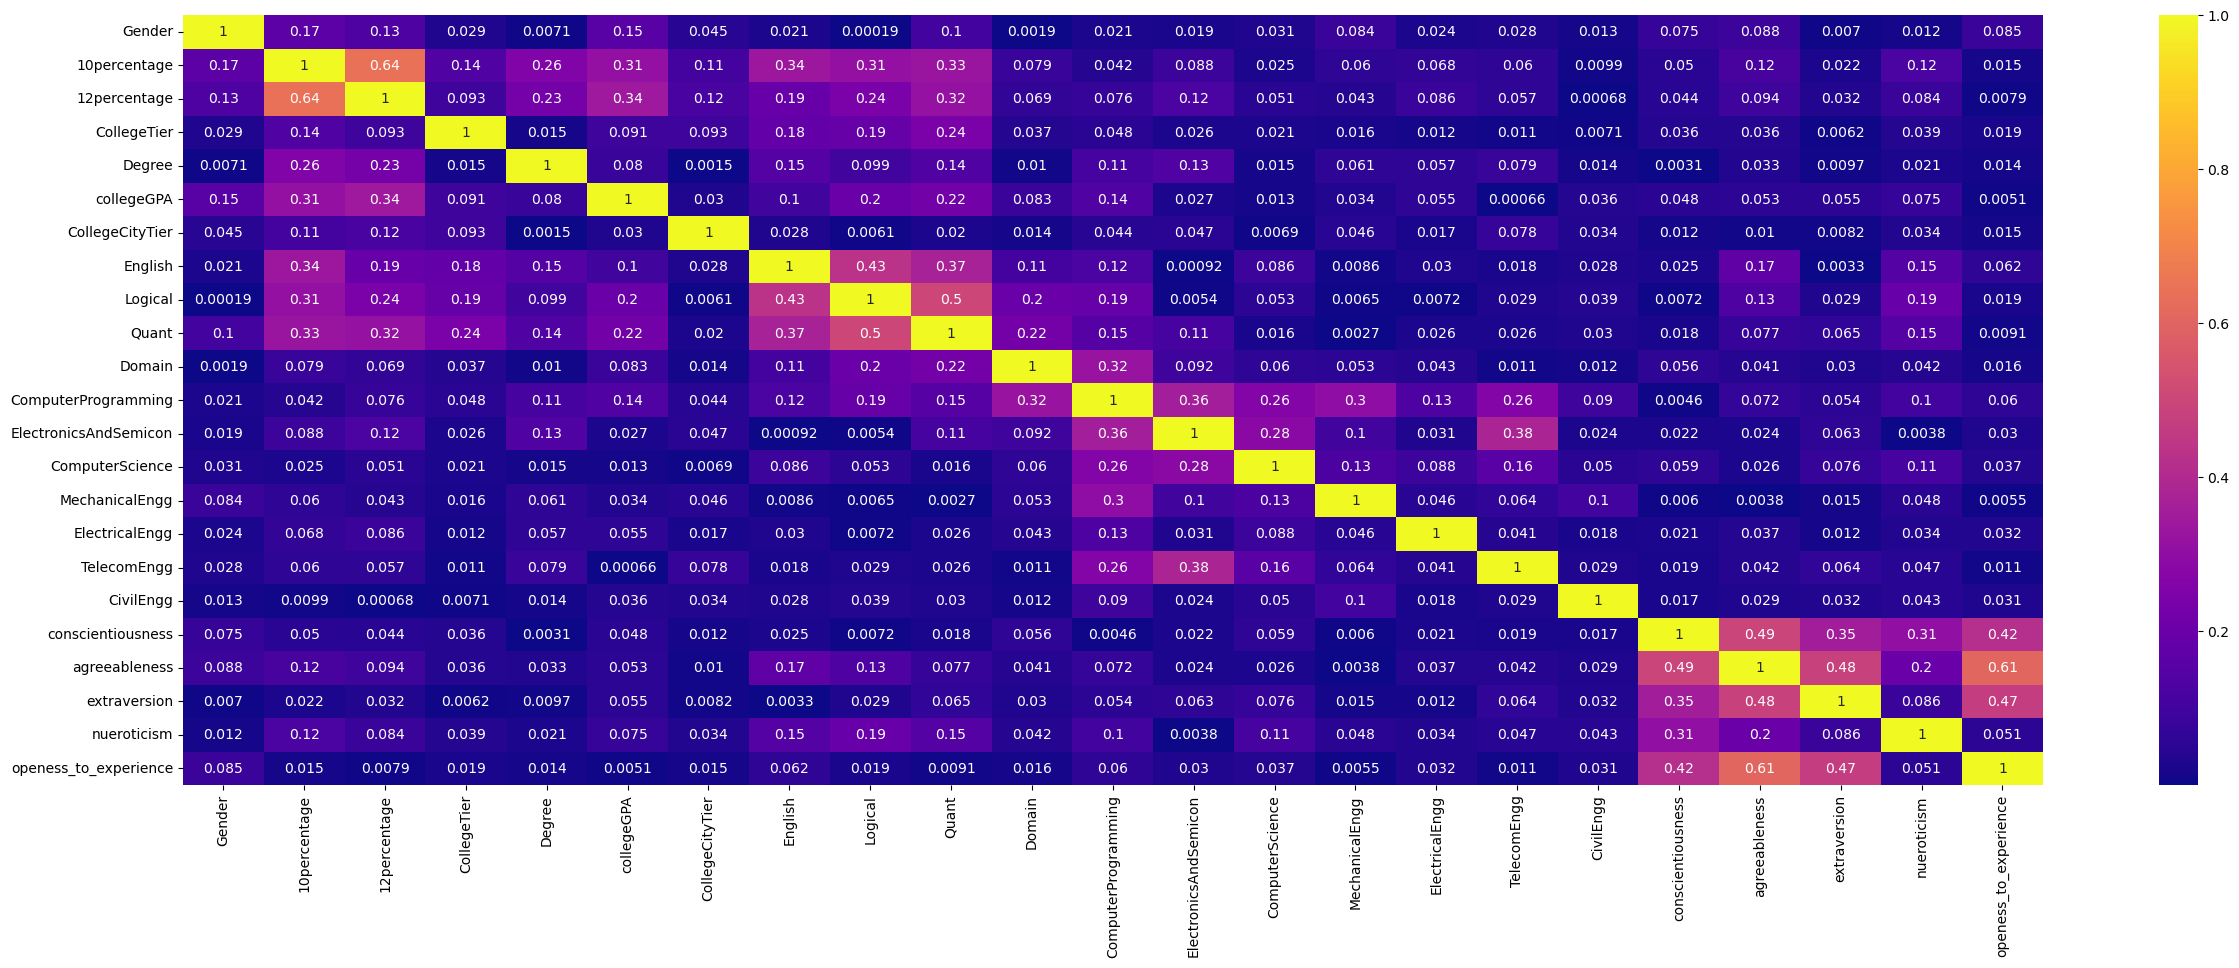
\includegraphics[width=\textwidth]{image/heatmap.png}
    \caption{Ma trận tương quan giữa các cột trong yêu cầu 1d}
    \label{fig:1d_corr}
\end{figure}

\subsubsection{Hàm pandas.corr}
\noindent
\textbf{Input:} Các tham số để tùy chỉnh cách tính ma trận tương quan. \\
\textbf{Output:} DataFrame chứa ma trận tương quan giữa các cột.
\paragraph{Mô tả:}

Ma trận tương quan (correlation matrix) là một ma trận vuông chứa các hệ số tương quan giữa nhiều biến. Mỗi ô trong bảng cho biết mối tương quan giữa hai biến cụ thể. Ma trận tương quan thường được sử dụng để tóm tắt dữ liệu, làm đầu vào cho phân tích nâng cao hơn và làm chẩn đoán cho phân tích nâng cao

Một số điểm cần lưu ý khi đọc ma trận tương quan:
\begin{itemize}
  \item Các hệ số tương quan trên đường chéo của bảng đều bằng 1 vì mỗi biến hoàn toàn tương quan với chính nó.
  \item Chỉ một nửa của ma trận tương quan cần được hiển thị vì nửa còn lại của các hệ số tương quan trong ma trận là dư thừa và không cần thiết.
  \item Ta có thể tô màu ma trận tương quan sẽ được như một bản đồ nhiệt (sử dụng tham số \textit{cmap} trong hàm heatmap) để làm cho các hệ số tương quan dễ đọc hơn.
\end{itemize}

Trong đồ án này, phương pháp Pearson \cite{wikipediaPearsonCorrelation} được sử dụng để tính ma trận tương quan. Phương pháp này được sử dụng để đo lường mối quan hệ giữa hai biến ngẫu nhiên X và Y. Giá trị của hệ số tương quan Pearson nằm trong khoảng [-1, 1]. Hệ số tương quan bằng 1 nếu có mối quan hệ tuyến tính thuận hoàn hảo giữa hai biến, bằng -1 nếu có mối quan hệ tuyến tính nghịch hoàn hảo giữa hai biến. Hệ số tương quan bằng 0 nếu không có mối quan hệ tuyến tính giữa hai biến.

Công thức tính hệ số tương quan Pearson giữa hai biến X và Y:
\begin{equation}
    \text{r}_{\text{X,Y}} = \frac{\sum_{i=1}^{n} (x_i - \bar{x})(y_i - \bar{y})}{\sqrt{\sum_{i=1}^{n} (x_i - \bar{x})^2} \sqrt{\sum_{i=1}^{n} (y_i - \bar{y})^2}}
\end{equation}

Trong đó:
\begin{itemize}
    \item $\text{r}_{\text{X,Y}}$ là hệ số tương quan Pearson giữa hai biến X và Y.
    \item $x_i$ là giá trị của biến X tại điểm dữ liệu thứ i.
    \item $y_i$ là giá trị của biến Y tại điểm dữ liệu thứ i.
    \item $\bar{x}$ là giá trị trung bình của biến X.
    \item $\bar{y}$ là giá trị trung bình của biến Y.
    \item n là số lượng điểm dữ liệu.
\end{itemize}

Do ta cần quan tâm độ tương quan giữa hai đặc trưng chứ không quan tâm chúng có tương quan thuận hay nghịch, nên ta sẽ lấy giá trị tuyệt đối của hệ số tương quan Pearson để tính ma trận tương quan. Bằng cách gọi hàm \textit{abs()} trên DataFrame chứa ma trận tương quan, ta sẽ được ma trận tương quan giữa các cột như hình 

% Numpy
\subsubsection{Hàm numpy.linalg.inv}
\noindent
\textbf{Input:} Ma trận vuông cần tính ma trận nghịch đảo. \\
\textbf{Output:} Ma trận nghịch đảo của ma trận đầu vào.
\paragraph{Mô tả:}

Hàm \textit{numpy.linalg.inv} \cite{numpyNumpylinalginv} được sử dụng để tính ma trận nghịch đảo của ma trận vuông. Trong đồ án này, hàm này được sử dụng để tính ma trận nghịch đảo của ma trận $\text{A}^\text{T} \text{A}$ để tìm nghiệm của hệ phương trình tuyến tính $\text{x} = (\text{A}^\text{T} \text{A})^{-1} \text{A}^\text{T} \text{b}$ (hàm \textit{fit} trong class OLSLinearRegression tự cài đặt, song để tối ưu hoá thời gian tính toán, ta sẽ sử dụng hàm \textit{numpy.linalg.inv} để tính ma trận nghịch đảo thay vì tự cài đặt).

\subsubsection{Hàm numpy.ravel} \label{ravel}
\noindent
\textbf{Input:} Mảng NumPy được đọc theo thứ tự được chỉ định bởi tham số order và được đóng gói thành một mảng 1 chiều và được đọc theo thứ tự C. \\
\textbf{Output:} Mảng NumPy một chiều.
\paragraph{Mô tả:}

Trong numpy, tham số order được sử dụng để chỉ định cách mà các phần tử của một mảng được lưu trữ trong bộ nhớ C trong \textit{order='C'}, có nghĩa là mảng được lưu trữ theo thứ tự liên tục của C, hay chỉ số cuối cùng thay đổi nhanh nhất \cite{stackoverflowCOrder}. Điều này có nghĩa là khi bạn duyệt qua các phần tử của một mảng nhiều chiều theo thứ tự C, bạn sẽ duyệt qua các phần tử của chỉ số cuối cùng trước, sau đó tăng chỉ số kế cuối lên 1 và tiếp tục duyệt qua các phần tử của chỉ số cuối cùng, và cứ tiếp tục như vậy cho đến khi duyệt hết các phần tử của mảng.

Trong bài toán hồi quy tuyến tính, chúng ta cần tìm một ma trận trọng số self.w sao cho tổng bình phương sai số giữa giá trị dự đoán và giá trị thực tế là nhỏ nhất. Để làm được điều này, chúng ta cần biến đổi ma trận trọng số thành một vector có kích thước bằng với số lượng tham số trong mô hình. Hàm \textit{numpy.ravel()} \cite{numpyNumpyravel} giúp chúng ta thực hiện việc này một cách dễ dàng và nhanh chóng. Bằng cách sử dụng hàm này, chúng ta có thể tính toán tích vô hướng giữa vector trọng số và ma trận đầu vào X bằng cách nhân từng phần tử tương ứng và cộng lại bằng cách gọi hàm \textit{numpy.sum}. Cuối cùng ta thu được giá trị dự đoán cho từng quan sát trong ma trận đầu vào X.

Hàm \textit{numpy.ravel} cũng được sử dụng trong hàm \ref{mae} để làm phẳng các mảng đầu vào y và y\_hat thành các mảng 1 chiều. Điều này cho phép tính toán trực tiếp sự khác biệt tuyệt đối giữa các phần tử tương ứng của hai mảng bằng cách trừ chúng và lấy giá trị tuyệt đối. Sau đó, giá trị trung bình của các sự khác biệt tuyệt đối được tính toán bằng hàm \textit{numpy.mean} để trả về giá trị lỗi trung bình tuyệt đối (MAE) giữa hai mảng.

\subsubsection{Hàm numpy.sum}
\noindent
\textbf{Input:} Mảng NumPy cần tính tổng, cột cần tính tổng \\
\textbf{Output:} Hàm này trả về kết quả là tổng của các phần tử trong mảng đầu vào theo các tham số đã xác định. Hàm có thể xử lý các mảng có kích thước và chiều khác nhau, và có thể thực hiện broadcasting nếu các kích thước tương thích.
\paragraph{Mô tả:}

Hàm \textit{numpy.sum} \cite{numpyNumpysum} được sử dụng để tính tổng các phần tử trong mảng. Trong đồ án này, hàm này được sử dụng để tính tổng các phần tử trong mảng đầu vào X bằng cách nhân từng phần tử tương ứng của vector trọng số và ma trận đầu vào X và cộng lại. Cuối cùng ta thu được giá trị dự đoán cho từng quan sát trong ma trận đầu vào X.
 
\subsubsection{Hàm numpy.mean} \label{mean}
\noindent
\textbf{Input:} Mảng NumPy cần tính trung bình, cột cần tính trung bình \\
\textbf{Output:} Hàm này trả về kết quả là trung bình của các phần tử trong mảng đầu vào theo các tham số đã xác định. Hàm có thể xử lý các mảng có kích thước và chiều khác nhau, và có thể thực hiện broadcasting nếu các kích thước tương thích.
\paragraph{Mô tả:}
Hàm \textit{numpy.mean} \cite{numpyNumpymean} được sử dụng để tính giá trị trung bình của các phần tử trong mảng. Trong đồ án này, hàm này được sử dụng để tính giá trị trung bình của các sự khác biệt tuyệt đối giữa các phần tử tương ứng của hai mảng bằng cách trừ chúng và lấy giá trị tuyệt đối. Sau đó, giá trị trung bình của các sự khác biệt tuyệt đối được tính toán bằng hàm \textit{numpy.mean} để trả về giá trị lỗi trung bình tuyệt đối (MAE) giữa hai mảng.

\subsubsection{Hàm numpy.triu}
\noindent
\textbf{Input:} Mảng NumPy cần tìm ma trận tam giác trên, kích thước của ma trận tam giác trên \\
\textbf{Output:} Mảng NumPy chứa ma trận tam giác trên của mảng đầu vào.
\paragraph{Mô tả:}
Hàm này trả về một bản sao của mảng đầu vào với các phần tử dưới đường chéo thứ k bị đưa về 0. Đối với các mảng có số chiều lớn hơn 2, triu sẽ áp dụng cho hai trục cuối cùng \cite{numpyNumpytriu}.

\subsubsection{Hàm numpy.where}
\noindent
\textbf{Input:} Mảng NumPy cần tìm vị trí, giá trị cần tìm vị trí \\
\textbf{Output:} Mảng NumPy chứa các vị trí của giá trị cần tìm.
\paragraph{Mô tả:}

Hàm \textit{numpy.where} \cite{numpyNumpywhere} được sử dụng để lọc các phần tử của một mảng dựa trên một điều kiện cho trước. Cụ thể hơn, \textcolor{red}{\textit{np.triu(np.ones(corr\_matrix.shape), k=1).astype(bool)}} sẽ tạo ra một mảng có cùng kích thước với corr\_matrix, trong đó các phần tử nằm trên đường chéo chính (k=1) sẽ có giá trị là True, còn các phần tử còn lại có giá trị là False.

Sau đó, mảng này được sử dụng như một mặt nạ để lọc các phần tử của corr\_matrix bằng cách sử dụng phương thức where. Kết quả cuối cùng là một mảng mới chỉ chứa các phần tử nằm trên đường chéo chính của corr\_matrix, còn các phần tử còn lại sẽ bị loại bỏ (có giá trị là NaN).

Nói cách khác, đoạn code trên lọc ra ma trận tam giác trên của ma trận tương quan corr\_matrix, loại bỏ các phần tử nằm dưới đường chéo chính và giữ lại các phần tử nằm trên đường chéo chính.

\subsubsection{Hàm numpy.ones}
\noindent
\textbf{Input:} Kích thước của mảng, kiểu dữ liệu của mảng \\
\textbf{Output:} Mảng NumPy chứa các phần tử có giá trị là 1.
\paragraph{Mô tả:}

Hàm \textit{numpy.ones} \cite{numpyNumpyones} được sử dụng để tạo ra một mảng có kích thước và kiểu dữ liệu nhất định, trong đó các phần tử có giá trị là 1.

% Seaborn
\subsubsection{Hàm seaborn.heatmap}
\noindent
\textbf{Input:} Ma trận tương quan, các tham số để tùy chỉnh cách vẽ heatmap. \\
\textbf{Output:} Biểu đồ heatmap.
\paragraph{Mô tả:}

Hàm \textit{seaborn.heatmap} \cite{pydataSeabornheatmap} được sử dụng để vẽ heatmap từ các đối tượng DataFrame hoặc numpy array, cũng như điều chỉnh các thuộc tính như bản đồ màu, khoảng giá trị, nhãn và tiêu đề. Heatmap là thành phần không thể thiếu để tìm hiểu mối quan hệ giữa các biến trong bộ dữ liệu và là tiền đề để thực hiện tìm mô hình cho yêu cầu 1d.

Tham số \textit{annot} trong hàm \textit{sns.heatmap} được sử dụng để kiểm soát việc hiển thị giá trị của các ô trong biểu đồ heatmap. Nếu \textit{annot=True}, thì giá trị của mỗi ô sẽ được hiển thị bên trong ô đó.

Biểu đồ heatmap với ma trận tương quan \text{corr\_matrix}, sử dụng bản đồ màu plasma, và hiển thị giá trị của mỗi ô bên trong ô đó. Nếu tham số này là False, thì giá trị của mỗi ô sẽ không được hiển thị bên trong ô đó, chỉ hiển thị các màu tương ứng với giá trị của ô đó.

% Sklearn
\subsubsection{Hàm sklearn.model\_selection.KFold}
\noindent
\textbf{Input:} Số lượng fold, các tham số để tùy chỉnh cách chia dữ liệu. \\
\textbf{Output:} Các chỉ số để chia dữ liệu thành các fold.
\paragraph{Mô tả:} 
Chiến lược phổ biến nhất trong học máy là chia tập dữ liệu thành tập huấn luyện và tập kiểm tra. Tỷ lệ chia có thể là 70:30 hoặc 80:20 \cite{r1}. Một trong số những phương pháp là sử dụng k-fold Cross Validation. \cite{mediumCrossValidationUsing}

Trong đồ án này, hàm \textit{sklearn.model\_selection.KFold} \cite{scikitlearnSklearnmodel} được sử dụng để chia dữ liệu thành các fold. Hàm này có thể nhận thêm các tham số để tùy chỉnh cách chia dữ liệu, nhưng trong đồ án này ta giữ nguyên các tham số khác xem như mặc định, chỉ tùy chỉnh số lượng fold, kiểu chia dữ liệu và trộn dữ liệu trước khi chia (lần lượt các tham số \textit{n\_splits}, \textit{shuffle} và \textit{random\_state}). Tham số \textit{n\_splits} được sử dụng để chỉ định số lượng fold (k = 20 với các yêu cầu 1b, 1c, 1d), tham số \textit{shuffle} được sử dụng để chỉ định cách chia dữ liệu, và tham số \textit{random\_state} được sử dụng để chỉ định cách trộn dữ liệu trước khi chia.

Tham số \textit{shuffle} được sử dụng để chỉ định cách chia dữ liệu. Nếu \textit{shuffle=True}, thì dữ liệu sẽ được trộn ngẫu nhiên trước khi chia. Nếu \textit{shuffle=False}, thì dữ liệu sẽ không được trộn ngẫu nhiên trước khi chia. Trong đồ án này, ta sử dụng \textit{shuffle=True} để trộn dữ liệu ngẫu nhiên trước khi chia.

Đến với tham số \textit{random\_state}, nếu \textit{random\_state=None}, thì mỗi lần chạy hàm \textit{KFold} sẽ cho ra kết quả khác nhau. Trên thực tế, việc truyền bất kì số nguyên nào (kể cả số 0) thì cũng không thành vấn đề. Đây là một random seed trong thuật toán random của máy tính. \cite{wikipediaRandomSeed} Các thí nghiệm có cùng random seed và cùng các tham số khác sẽ cho ra kết quả giống nhau. 42 là một con số đến từ cuốn sách Hướng dẫn du lịch vũ trụ. Câu trả lời cho cuộc sống vũ trụ và mọi thứ và được coi là một trò đùa. Nó không có ý nghĩa khác ngoài việc là một con số ngẫu nhiên. \cite{stackoverflowRandomState} Trong đồ án này, ta sử dụng \textit{random\_state=42} để đảm bảo kết quả của các thí nghiệm là nhất quán.

Việc chia dữ liệu thành k phần giúp chúng ta có thể kiểm tra độ chính xác và ổn định của mô hình trên nhiều tập dữ liệu khác nhau, tránh hiện tượng quá khớp (overfitting) hoặc thiếu khớp (underfitting) mô hình. Việc lựa chọn giá trị k trong k-fold cross validation là tùy thuộc vào nhiều yếu tố. Một giá trị k lớn sẽ cho phép mô hình được huấn luyện trên nhiều dữ liệu hơn, nhưng cũng sẽ tăng thời gian tính toán. Một giá trị k nhỏ sẽ giảm thời gian tính toán, nhưng cũng có thể làm tăng sai số trong việc đánh giá hiệu suất của mô hình. \cite{stackexchangeChoiceKfold}

% IPython
\subsubsection{Hàm IPython.display.Latex}
\noindent
\textbf{Input:} Chuỗi kí tự cần hiển thị ở dạng \LaTeX. \\
\textbf{Output:} Hiển thị chuỗi kí tự ở dạng \LaTeX.

\subsection{Hàm tự cài đặt}
\subsubsection{Hàm OLSLinearRegression.fit} \label{fit}
\noindent
\textbf{Input:} Ma trận chứa các giá trị của đặc trưng, y là một vector chứa các giá trị của biến mục tiêu. \\
\textbf{Output:} Chính nó (self) để có thể gọi phương thức khác trên cùng đối tượng OLSLinearRegression.
\paragraph{Mô tả:}

Hàm này sử dụng phương pháp bình phương nhỏ nhất để tính toán trọng số \textit{w} cho mô hình tuyến tính. Đầu tiên, nó tính toán ma trận giả nghịch đảo của ma trận $\text{A}^\text{T} \text{A}$ bằng hàm \textit{numpy.linalg.inv} (thay vì tự cài đặt để tối ưu hoá thời gian tính toán). 

Mục đích hàm fit của lớp OLSLinearRegression là tìm ra ma trận trọng số \textit{w} ứng với mô hình tuyến tính. Để làm được điều này, ta cần giải hệ phương trình tuyến tính $\text{A}^\text{T} \text{A} \textit{w} = \text{A}^\text{T} \text{b}$ để tìm ra giá trị của \textit{w}. Để giải hệ phương trình này, ta nhân cả hai vế của phương trình với ma trận nghịch đảo của ma trận $\text{A}^\text{T} \text{A}$, ta được $\textit{w} = (\text{A}^\text{T} \text{A})^{-1} \text{A}^\text{T} \text{b}$. Do đó, ta sẽ tính ma trận nghịch đảo của ma trận $\text{A}^\text{T} \text{A}$ bằng hàm \textit{numpy.linalg.inv} và nhân với ma trận $\text{A}^\text{T} \text{b}$ để tìm ra giá trị của \textit{w}.

\subsubsection{Hàm OLSLinearRegression.predict}
\noindent
\textbf{Input:} Ma trận chứa các giá trị của đặc trưng. \\
\textbf{Output:} Mảng NumPy chứa các giá trị dự đoán.
\paragraph{Mô tả:} 
Trong hàm \textit{predict}, ta tính toán giá trị dự đoán bằng cách nhân ma trận X với vector trọng số w (được tính toán trong hàm \hyperref{fit}{fit}) và cộng các giá trị lại với nhau theo chiều thứ nhất (axis=1) để thu được một vector kết quả. Cụ thể, ta sử dụng phép toán \textcolor{red}{\textit{np.sum(self.w.ravel() * X, axis=1)}} để thực hiện việc này.

Sở dĩ ta phải gọi hàm \textit{ravel} được sử dụng để chuyển đổi vector trọng số \textit{w} thành một mảng 1 chiều liên tục trước khi thực hiện phép nhân với ma trận đầu vào \textit{X}. Điều này cần thiết để đảm bảo rằng kích thước của \textit{w} và \textit{X} phù hợp với nhau và phép nhân. Trái lại, nếu không sử dụng hàm \textit{ravel}, vector trọng số \textit{w} có kích thước không phù hợp và dẫn đến lỗi khi thực hiện phép nhân.

\subsubsection{Hàm OLSLinearRegression.get\_params}
\noindent
\textbf{Input:} Không có. \\
\textbf{Output:} Mảng NumPy chứa các giá trị của vector trọng số \textit{w}.
\paragraph{Mô tả:}

Hàm \textit{get\_params} được sử dụng để trả về các giá trị của vector trọng số \textit{w}. Mô hình OLSLinearRegression sau khi được huấn luyện sẽ có một vector trọng số \textit{w} duy nhất, và hàm \textit{get\_params} được sử dụng để trả về các giá trị của vector trọng số này.

\subsubsection{Hàm mae} \label{mae}
\noindent
\textbf{Input:} Vector chứa các giá trị thực tế từ tập dữ liệu cho trước, vector chứa các giá trị dự đoán tính được từ mô hình. \\
\textbf{Output:} Giá trị lỗi trung bình tuyệt đối (MAE).
\paragraph{Mô tả:}

Phương pháp bình phương tối thiểu khi sử dụng để tìm mô hình tuyến tính sẽ tìm ra mô hình có giá trị trung bình của tổng bình phương sai số là nhỏ nhất.  Tuy nhiên, trong thực tế, chúng ta thường quan tâm đến giá trị trung bình của tổng sai số tuyệt đối, hay còn gọi là lỗi trung bình tuyệt đối (MAE). MAE được tính bằng cách lấy giá trị tuyệt đối của sự khác biệt giữa các giá trị thực tế và giá trị dự đoán, sau đó lấy giá trị trung bình của các sự khác biệt tuyệt đối này.

Trong hàm mae, ta sử dụng hàm \textit{numpy.ravel} để làm phẳng các mảng đầu vào y và y\_hat thành các mảng 1 chiều. Điều này cho phép tính toán trực tiếp sự khác biệt tuyệt đối giữa các phần tử tương ứng của hai mảng bằng cách trừ chúng và lấy giá trị tuyệt đối. Sau đó, giá trị trung bình của các sự khác biệt tuyệt đối được tính toán bằng hàm \textit{numpy.mean} để trả về giá trị lỗi trung bình tuyệt đối (MAE) giữa hai mảng.

\subsubsection{Hàm latex\_text}
\noindent
\textbf{Input:} Mảng NumPy chứa các tham số của mô hình tuyến tính, từ điển chứa các tên cột tương ứng với các tham số trong mảng NumPy. \\
\textbf{Output:} Hiển thị chuỗi kí tự ở dạng \LaTeX.
\paragraph{Mô tả:}

Hàm latex\_text có hai đầu vào là params và dict. Đầu vào params là một mảng numpy chứa các tham số của mô hình tuyến tính, trong khi đầu vào dict là một từ điển chứa các tên cột tương ứng với các tham số trong params. Hàm này trả về một chuỗi LaTeX biểu diễn phương trình tuyến tính của mô hình dựa trên các tham số và tên cột được cung cấp.

Trong hàm này, ta bắt đầu bằng cách khởi tạo chuỗi text với giá trị ban đầu là phần đầu của phương trình LaTeX: Hàm latex\_text có hai đầu vào là params và dict. Đầu vào params là một mảng numpy chứa các tham số của mô hình tuyến tính, trong khi đầu vào dict là một từ điển chứa các tên cột tương ứng với các tham số trong params. Hàm này trả về một chuỗi LaTeX biểu diễn phương trình tuyến tính của mô hình dựa trên các tham số và tên cột được cung cấp.

\subsubsection{Hàm kfold\_cross\_model}
\noindent
\textbf{Input:} Mảng NumPy chứa các giá trị của đặc trưng, mảng NumPy chứa các giá trị của biến mục tiêu, đối tượng KFold, mảng để lưu trữ các giá trị MAE. \\
\textbf{Output:} Không có.
\paragraph{Mô tả:}

Trong hàm này, ta sử dụng vòng lặp để duyệt qua các phần chia của dữ liệu huấn luyện khi thực hiện phương pháp kfold cross validation. Mỗi phần tử của iterator là một tuple chứa hai mảng chỉ số: \textit{train\_index} và \textit{test\_index}. Mảng \textit{train\_index} chứa các chỉ số của phần huấn luyện, trong khi mảng \textit{test\_index} chứa các chỉ số của phần kiểm tra1.

Vòng lặp \textcolor{red}{\textit{for train\_index, test\_index in kf.split(X\_train\_np)}} được sử dụng để duyệt qua các phần chia của dữ liệu huấn luyện. Đối với mỗi phần chia, ta sử dụng chỉ số của phần huấn luyện và phần kiểm tra để trích xuất dữ liệu tương ứng từ X\_train\_np và y\_train\_np. Sau đó, ta có thể huấn luyện mô hình với dữ liệu huấn luyện đã trích xuất và đánh giá hiệu suất của mô hình trên dữ liệu kiểm tra. Cuối cùng, ta thêm giá trị MAE vào danh sách mae\_arr để lưu trữ kết quả. Nếu X\_train\_np là một vector 1 chiều, ta thêm một chiều mới vào cuối bằng cách sử dụng cú pháp [:, None]. Ngược lại, ta chỉ cần trích xuất dữ liệu bình thường. Sau đó, ta huấn luyện một mô hình hồi quy tuyến tính bằng cách sử dụng phương thức fit của class OLSLinearRegression với dữ liệu huấn luyện đã trích xuất. Ta sử dụng mô hình đã huấn luyện để dự đoán giá trị đầu ra cho phần kiểm tra của dữ liệu và tính toán giá trị MAE giữa giá trị thực tế và giá trị dự đoán. Cuối cùng, ta thêm giá trị MAE vào danh sách mae\_arr để lưu trữ kết quả.

Hàm này không có giá trị trả về, nhưng nó thay đổi nội dung của danh sách mae\_arr bằng cách thêm các giá trị MAE tính toán được trong quá trình kiểm định chéo.

\subsubsection{Hàm scientific\_notation\_converter}
\noindent
\textbf{Input:} Mảng chứa các trọng số của mô hình tuyến tính. \\
\textbf{Output:} Mảng chứa các trọng số của mô hình tuyến tính ở dạng ký hiệu khoa học với 3 chữ số thập phân.
\paragraph{Mô tả:}

Trong đồ án yêu cầu ta phải trình bày mô hình dự đoán mức lương với tham số được làm tròn 3 chữ số thập phân. Ta có thể sử dụng hàm \textit{round} trong phương thức \textit{get\_params}. Song nếu làm tròn ngay từ bước huấn luyện, ta sẽ mất đi độ chính xác của mô hình. Do đó, ta sẽ sử dụng hàm \textit{scientific\_notation\_converter} để chuyển đổi các trọng số của mô hình.

Trong hàm này, ta sử dụng kỹ thuật list comprehension để duyệt qua các phần tử trong params và chuyển đổi chúng thành dạng ký hiệu khoa học (scientific notation). Đối với mỗi phần tử x trong params, ta chuyển đổi nó thành số thực bằng cách sử dụng hàm float(x), sau đó định dạng nó thành chuỗi ký hiệu khoa học với 3 chữ số thập phân bằng cách sử dụng phương thức format: \textit{"\{:.3f\}".format(float(x))}. Kết quả cuối cùng là một danh sách mới chứa các chuỗi ký hiệu khoa học tương ứng với các phần tử trong params.

\section{Đánh giá kết quả mô hình}
% \subsubsection{Các bước thực hiện}
% \subsubsection{Công thức hồi quy}
% \subsubsection{Kết quả mô hình}
% \subsubsection{Nhận xét}

Trước khi thực hiện tìm mô hình hồi quy tuyến tính cho tất cả yêu cầu đề bài, ta cần đọc dữ liệu từ \textit{train.csv} và \textit{test.csv} ứng với tập dữ liệu huấn luyện (\textbf{train}) và tập dữ liệu kiểm tra (\textbf{test}), đồng thời xử lý DataFrame vừa đọc được để nhận biết đâu là tập các đặc trưng (\textbf{X}) và đâu là tập biến mục tiêu (\textbf{y}). Sau đó, ta sẽ chia tập dữ liệu huấn luyện thành hai phần: tập huấn luyện (\textbf{X\_train}, \textbf{y\_train}) và tập kiểm tra (\textbf{X\_test}, \textbf{y\_test}). Do tập mục tiêu là cố định (Salary ứng với \textbf{y\_train} và \textbf{y\_test}), nên ta dùng chung hai tập này cho các câu 1a, 1b, 1c, 1d. 

Sở dĩ phải chuyển về NumPy array với tất cả DataFrame vừa đọc được là vì khi thực hiện yêu cầu tìm đặc trưng tốt nhất trong số các đặc trưng (yêu cầu 1b, 1c), ma trận đặc trưng \textit{X} chỉ có 1 cột, nên khi thực hiện các phép toán trên ma trận, ta cần mở rộng 1 chiều mới 

\subsection{Yêu cầu 1a}
\subsubsection{Các bước thực hiện}
\begin{enumerate}
  \item Thực hiện lấy 11 đặc trưng đầu tiên đề bài cung cấp.
  \item Thực hiện chia tập dữ liệu huấn luyện thành hai phần: tập huấn luyện (\textbf{X\_1a\_train}, \textbf{y\_train}) và tập kiểm tra (\textbf{X\_test}, \textbf{y\_test}).
  \item 
\end{enumerate}
\subsubsection{Công thức hồi quy}
\subsubsection{Kết quả mô hình}
\subsubsection{Nhận xét}

\subsection{Yêu cầu 1b}

\subsection{Yêu cầu 1c}

\subsection{Yêu cầu 1d}

\newpage
\printbibliography[heading=mybibintoc]

\end{document}